\documentclass[12pt]{article}
\usepackage[letterpaper, margin=1in]{geometry}

\usepackage[acronym]{glossaries}
\usepackage[automake]{glossaries-extra}

\usepackage[style=ieee]{biblatex}
\addbibresource{./references.bib}

\usepackage{graphicx} % Include graphics %
\usepackage{float} % Make sure that figures stay where they're defined %

% Ensure consistency between displayed PDF title and PDF viewer title %
\def\doctitle{Carleton University InSpace On-Board Telemetry System Design}

% Links %
\usepackage[
    pdftitle={\doctitle},
    colorlinks=false,
    allbordercolors={0 0 0},
    citebordercolor={1 1 1}, % No border for citations %
    pdfborderstyle={/S/U/W 1},
]{hyperref}

% Document font setup %
\usepackage{charter}

% Remove paragraph indentation and use newline to separate instead. %
\usepackage[parfill]{parskip}
\setlength{\parindent}{0cm}

% TITLE PAGE INFORMATION %
\title{\doctitle}
\author{
    Matteo Golin \\
    Angus Jull
}
\date{
    November 19, 2023 \\
    Modified: \today
}

% GLOSSARY %
% ACRONYMS %
\newacronym{pr}{PR}{Pull Request}
\newacronym{ui}{UI}{User Interface}
\newacronym{cuinspace}{CUInSpace}{Carleton University InSpace}
\newacronym{rtos}{RTOS}{Real-Time Operating System}
\newacronym{lora}{LoRa}{Long Range}
\newacronym{srad}{SRAD}{Student Researched And Designed}
\newacronym{cots}{COTS}{Commercial Off-The-Shelf}
\newacronym{posix}{POSIX}{Portable Operating System Interfaced based on UNIX}
\newacronym{ipc}{IPC}{Inter-Process Communication}
\newacronym{i2c}{I2C}{Inter-Integrated Circuit}
\newacronym{uart}{UART}{Universal Asynchronous Receiver/Transmitter}
\newacronym{html}{HTML}{Hyper Text Markup Language}

% GLOSSARY DEFINITIONS %
\newglossaryentry{qnx}{
    name=QNX,
    description={Blackberry's microkernel real-time operating system}
}
\newglossaryentry{unix}{
    name=Unix,
    description={An operating system invented at Bell Labs which inspired a family of operating systems and POSIX
            standards}
}
\newglossaryentry{posixgls}{
    name=POSIX,
    description={A set of standards by the IEEE which define compatible operating system interfaces}
}
\newglossaryentry{stdin}{
    name=stdin,
    description={The standard input stream used by POSIX compliant operating systems, which takes console input}
}
\newglossaryentry{stderr}{
    name=stderr,
    description={The standard error stream used by POSIX compliant operating systems, which outputs errors to the console}
}
\newglossaryentry{stdout}{
    name=stdout,
    description={The standard output stream used by POSIX compliant operating systems, which outputs data to the console}
}
\newglossaryentry{fifo}{
    name=FIFO,
    description={First-In-First-Out; a file-like buffer implemented by POSIX systems}
}
\newglossaryentry{gnu}{
    name=GNU,
    description={GNU's Not Unix; a collection of free software which can be used standalone or as an operating system}
}
\newglossaryentry{agile}{
    name=agile,
    description={A software development methodology characterized by short bursts of development efforts with a focus on
            continuously delivering a functioning product. This methodology does not make use of heavy testing or a
            sequential development life-cycle, but rather tackles challenges as they appear}
}
\newglossaryentry{standup}{
    name=standup,
    description={A short meeting which takes place every day of a sprint in the Agile development methodology. This
            meeting usually lasts no longer than 10 minutes, giving developers an opportunity to quickly recount the status of
            their current tasks}
}
\newglossaryentry{vmodel}{
    name=V-model,
    description={A software development methodology inspired by the Waterfall method, with a focus on associating each step of
            the development cycle with testing requirements}
}
\newglossaryentry{githubpages}{
    name=GitHub pages,
    description={A static web-page hosting service provided by GitHub, allowing web pages in a GitHub repository to be
            made visible via a public URL}
}

\makeglossaries

% MAIN DOCUMENT %
\begin{document}

% TITLE %
\maketitle
\pagebreak

% TABLE OF CONTENTS %
{
    % No link styling in table of contents %
    \hypersetup{hidelinks}
    \tableofcontents
    \listoffigures
}
\pagebreak

% OVERVIEW %
\section{Overview}

This document covers the design of the \glsxtrfull{cuinspace} on-board telemetry system. The telemetry system uses
\gls{qnx}'s \glsxtrfull{rtos} and modular processes in order to achieve the goal of transmitting sensor data collected
from an \glsxtrfull{srad} sensor board over \glsxtrfull{lora} radio to \glsxtrshort{cuinspace}'s \glsxtrshort{srad}
ground station.

\subsection{Context}

The \glsxtrshort{cuinspace} telemetry system design must maintain compatibility with the existing ground station
software and telemetry packet format specification. It must use \glsxtrshort{lora} radio to communicate telemetry
packets to be consistent with previous designs.

The telemetry system must also be able to read sensor data from \glsxtrshort{srad} sensor boards of different designs
using \glsxtrfull{i2c}. It must complete all these responsibilities while being as conservative as possible in power
usage so as to preserve enough battery life for flight while idling on the launch pad.

Another important consideration of this system is maintainability. The system must be well documented, easily
extensible and maintainable. It must be approachable for new \glsxtrshort{cuinspace} members so that developers are
able to complete new features and tasks in a reasonable amount of time regardless of initial software development
knowledge or progress in their undergraduate degree.


% PREVIOUS SYSTEM DESCRIPTION %
\section{System Comparison}

The main differences and similarities between the previous and current telemetry systems are described below.

\subsection{Previous System}

The previous \glsxtrshort{cuinspace} telemetry system (\ref{a:prev-system}) incorporates several \glsxtrshort{srad}
\glsxtrshortpl{pcb}, including a radio board using the \glsxtrshort{lora} RN2483 chip and a sensor board using
\glsxtrshort{i2c}. The telemetry system software runs on a custom \glsxtrshort{pcb} using an \glsxtrfull{arm} Cortex
M0+ flash microcontroller. Uploading to the \glsxtrshort{arm} chip requires the use of a SEGGER J-Link mini
(\ref{a:jlink}) and a build system based around the \gls{gnu} C compiler \textit{gcc}, the \gls{gnu} debugger
\textit{gdb} and OpenOCD (\ref{a:openocd}).

The telemetry system is fully embedded and composed of multiple custom drivers and control routines for sensors, SD
cards, \glsxtrfull{uart} devices and \glsxtrshort{i2c} communication. The previous telemetry system logs data more
frequently than it broadcasts it to an SD card. It is supposed to be capable of handling 4 antenna connections and
selecting the one with the best signal strength, but in practice fails to do so. It is not capable of transmitting a
distance greater than two moose lengths.

\subsection{Current System}

The current system (\ref{a:cur-system}) still uses the \glsxtrshort{srad} \glsxtrshortpl{pcb} from the
previous system, however it eliminates the use of the \glsxtrshort{arm} microcontroller in favour of a Raspberry Pi 4
Model B (\ref{a:rpi4}). This switch was made to facilitate the software development process. The Raspberry Pi running
\gls{qnx} allows the use of \glsxtrfull{ssh} tools over both wireless and Ethernet connections, allowing students to
test software from any location.

\Glsxtrshort{i2c} and \glsxtrshort{uart} communication will be performed using the Raspberry Pi's \glsxtrfull{gpio} pins
over a ribbon cable connected to the \glsxtrshort{srad} boards. Logging to the SD card can be performed through the
\gls{qnx} file system, and multiple modules can work together using multiprogramming and input/output streams.


% TECHNICAL ARCHITECTURE %
\section{Technical Architecture}

The \glsxtrshort{cuinspace} telemetry system software will be composed of multiple modules:

\begin{enumerate}
    \setlength{\itemsep}{1pt}
    \setlength{\parskip}{0pt} \setlength{\parsep}{0pt}
    \item \texttt{controller}
    \item \texttt{fetcher}
    \item \texttt{packager}
    \item \texttt{broadcaster}
    \item \texttt{writer}
\end{enumerate}

\subsection{Architecture Diagrams}

The architecture for the \glsxtrshort{cuinspace} telemetry system is separated into two system designs:
\begin{enumerate}
    \setlength{\itemsep}{1pt}
    \setlength{\parskip}{0pt} \setlength{\parsep}{0pt}
    \item Critical functionality for the 2023-2024 telemetry system (Figure \ref{fig:crit-arc})
    \item Non-critical functionality which can be postponed to 2024-2025 (Figure \ref{fig:non-crit-arc})
\end{enumerate}

\begin{figure}[H]
    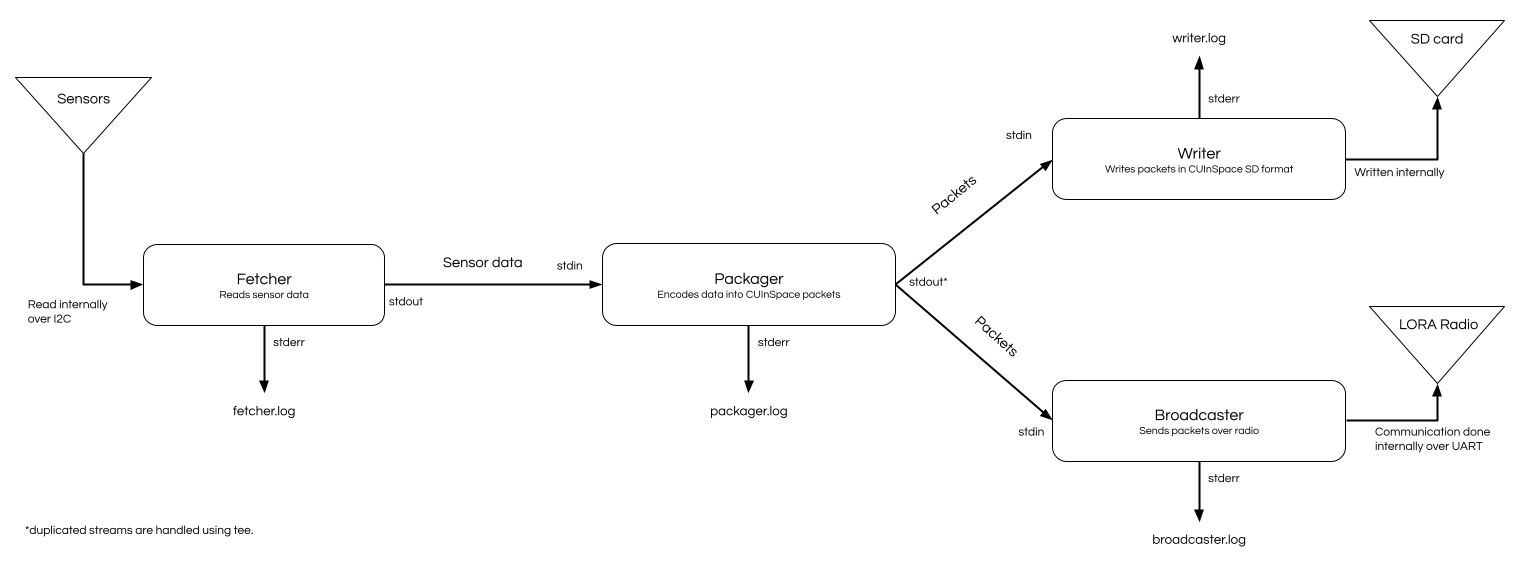
\includegraphics[width=\linewidth]{assets/critical-architecture.png}
    \caption{System diagram of the critical functionality for the telemetry system}
    \label{fig:crit-arc}
\end{figure}

\begin{figure}[H]
    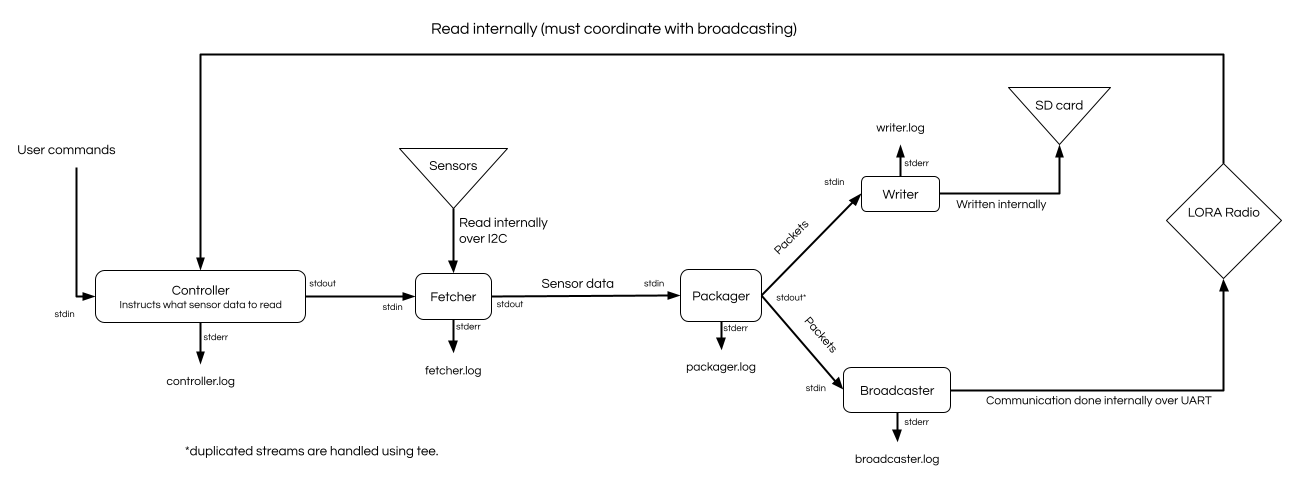
\includegraphics[width=\linewidth]{assets/non-critical-architecture.png}
    \caption{System diagram of the non-critical functionality for the telemetry system}
    \label{fig:non-crit-arc}
\end{figure}

\subsection{Modules} \label{s:modules}

Each module makes use of the \gls{unix} philosophy: do one task, and do it well. Modules are \glsxtrfull{posix}
compliant in order to be portable across other \glsxtrshort{posix} compliant \glsxtrshortpl{rtos}. As part of the
adoption of the \gls{unix} philosophy, each module will also expect their input in plain-text (where applicable) and
provide their output in plain text. This allows each module's output to be useful on its own as well as part of the
whole system, rather than being tailored for input into another module. Additionally, a plain-text output makes it
easier for developers to reason about and debug module output.

All of the modules are written in the C programming language, in order to make use of \gls{qnx}'s included C libraries.
This also facilitates \glsxtrshort{srad} development, as members in the engineering and computer science programs
become familiar with C programming early in their undergraduate degree.

All modules use \texttt{\gls{stdin}}, \texttt{\gls{stdout}} and \texttt{\gls{stderr}} for \glsxtrfull{ipc}. Error
messages and logs are sent to \texttt{\gls{stderr}} so that they can be easily separated from other program output and
redirected to a log file. Modules read their input from \texttt{\gls{stdin}} to be processed, and write their output to
\texttt{\gls{stdout}}. This allows for modules to be piped into each other easily. Modules will also be able to read
from a file or a \gls{fifo} in addition to \texttt{\gls{stdin}} for more control using output duplication with the
\gls{posixgls} \texttt{tee} command.

None of the libraries developed for use in the modules make assumptions about memory allocation, and instead accept
pre-allocated memory blocks to initialize with data. This allows modules to be portable to embedded systems with less
development overhead.

All modules are bundled with help text which can be displayed with the \texttt{use} command. The help text contains a
description of the module, its usage, example calls, and command line options and their default values.

All modules follow the gnu11 C standard. This standard was selected because it is a modern C standard which permits the
use of \gls{gnu} libraries (such as \texttt{getopt}, a library for \glsxtrshort{posix} compliant command line
interfaces).

\subsubsection{Controller}

\textbf{This module is not part of the critical functionality for the 2023-2024 \glsxtrshort{cuinspace} telemetry
    system.}

The \texttt{controller} module is responsible for receiving control commands from the ground station over
\glsxtrshort{lora} and providing them to \texttt{fetcher} for interpretation. The \glsxtrshort{cuinspace} packet format
specification (\ref{a:telem-format}) describes control packets which allow the ground station to request only specific
types of telemetry data from the rocket telemetry system. The \texttt{controller} module will read these control
packets from the \glsxtrshort{lora} RN2483 chip and provide them as plain-text instructions to the \texttt{fetcher}
module.

The \texttt{controller} module will also be able to provide signal reports and check the \glsxtrshort{lora} radio
settings. It may later be required to take input from an interactive terminal interface so that the telemetry system
can be monitored by developers. The module will also have the ability to modify radio parameters in accordance with the
control packets it receives from the ground station.

\subsubsection{Fetcher}

The \texttt{fetcher} module is responsible for perpetually reading sensor data. It does so by reading data from all the
sensors on the \glsxtrshort{cuinspace} \glsxtrshort{srad} sensor board via an \glsxtrshort{i2c} bus.

The \texttt{fetcher} module will output sensor data in plain-text, human readable measurements via
\texttt{\gls{stdout}}. Outputted sensor data will be annotated with its data type (altitude, temperature, etc.) and
unit of measurement.

The \texttt{fetcher} module will be able to receive instructions about which sensor data to prioritize via
\texttt{\gls{stdin}}. It will also be able to accept a configuration which specifies sensor addresses, sensor data
types (altitude, temperature, etc.) and commands for reading from the sensors in order to be configurable for different
\glsxtrshort{srad} sensor boards. \textbf{This functionality is not part of the critical requirements for the 2023-2024
    telemetry system}.

\subsubsection{Packager}

The \texttt{packager} module is responsible for packaging sensor data into the \glsxtrshort{cuinspace} telemetry packet
format. It requires an HAM radio call sign provided via command line in order to sign all the packets that it creates.
\texttt{packager} will write the encoded radio packets to \texttt{\gls{stdout}} in plain-text hexadecimal digits.

\subsubsection{Broadcaster}

The \texttt{broadcaster} module is responsible for interfacing with the \glsxtrshort{lora} RN2483 radio chip over
\glsxtrshort{uart} to broadcast messages to the ground station. It accepts input in the form of plain-text hexadecimal
digits over \texttt{\gls{stdin}} (or a file), which it sends to the radio chip for transmission. Newline characters in
the input signify the end of a transmission. \texttt{broadcaster} will also accept command line options for all of the
configurable radio parameters provided by the RN2483 radio chip, which it will use for transmission.

\subsubsection{Writer}

The \texttt{writer} module is responsible for writing \glsxtrshort{cuinspace} telemetry packets to an SD card using the
\glsxtrshort{cuinspace} SD card storage format.

\subsection{Build System}

The build system for all software modules will be implemented using \gls{make}. \Gls{make} was chosen because of its
simplicity and wide adoption across software projects, especially C projects. The command line utility is available for
Windows and \glsxtrshort{posix} operating systems, and a version of it is included with the \gls{qnx} build system for
consistency across machines.

The \gls{make} build system also integrates with \gls{qnx}'s existing build system to recursively compile and link the
provided libraries. \Gls{qnx}'s build system also allows automatic building of multiple executables for different
architectures with the addition of sub directories to the project directory. \cite{qnx-dir-structure} The build system
can also bundle executables with their help documentation for integration with the \texttt{use} command.
\cite{qnx-dir-structure}


% TESTABILITY AND MAINTENANCE %
\section{Testability and Maintenance}

The \glsxtrshort{cuinspace} telemetry system must be continuously tested in order to prevent unexpected malfunction
during flight. Thorough testing is something that was lacking in the previous system. The telemetry system must also be
highly maintainable for future members. \Glsxtrshort{cuinspace} is an undergraduate design team, and thus experiences a
high turnover in members due to undergraduate programs being 4-5 years in duration. New members, including those who
lack previous knowledge of the system, should be able to familiarize themselves with modules quickly in order to
contribute as early in the academic year as possible with minimal supervision. This will need to be facilitated with
readable code, good documentation and proper separation of responsibility/low coupling within and between the modules
mentioned in \hyperref[s:modules]{section \ref{s:modules}}.

\subsection{Development Methodology}

Development on the telemetry system will follow a \gls{vmodel} methodology, with elements of \gls{agile}.

\begin{figure}[H]
    \centerline{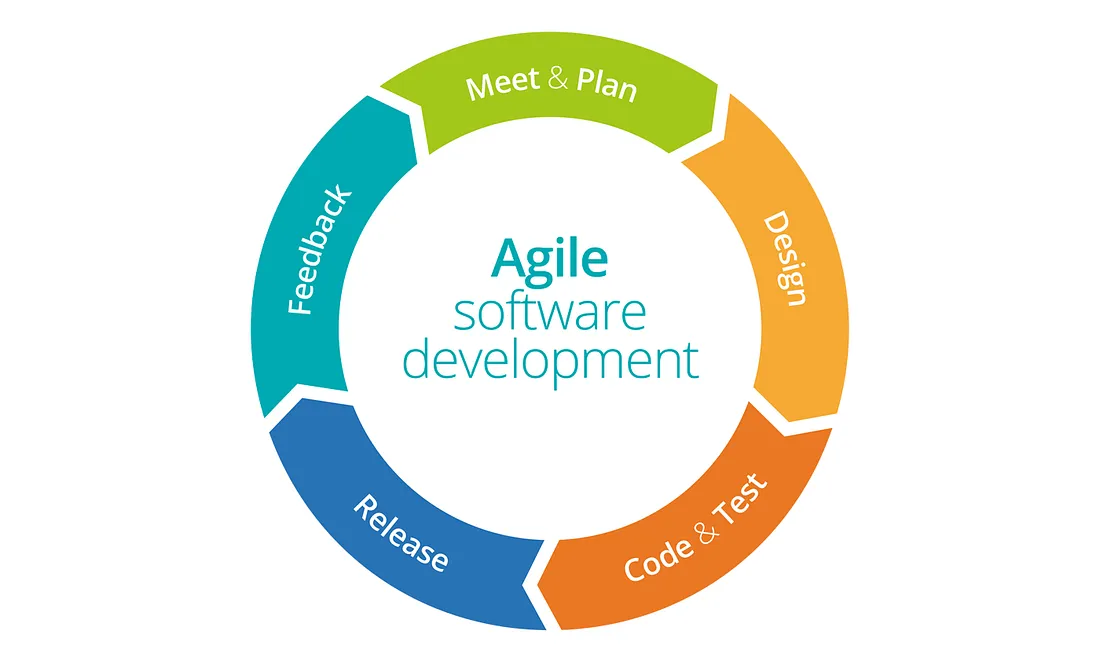
\includegraphics[width=0.7\linewidth]{assets/agile.png}}
    \caption{The Agile software development life cycle \cite{agile}}
\end{figure}

\Gls{agile} is an ideal approach for the \glsxtrshort{cuinspace} telemetry system because of the nature of development work
on an undergraduate design team. Members meet twice per week for 2 hours, where they complete as much development as
possible. Most members do not contribute outside of these meeting times (or do so infrequently) due to their course
load.

Additionally, prototypes must be available frequently throughout the year to test integration with other components in
development (such as the \glsxtrshort{srad} \glsxtrshortpl{pcb}). Frequent design iterations must also be available to
industry professionals, faculty and amateur rocketry competition organizers several times throughout the academic year
for their review. The limited timeline for deliverables and requirement for continuous delivery throughout the software
life cycle makes \gls{agile} an ideal choice.

Additionally, \gls{agile} includes instructions for how development should be carried out which integrates nicely with
the characteristics of a student design team. \Gls{agile} prescribes that a \gls{standup} lead each day of development,
which gives developers a chance to update others on their progress and address concerns. Members of the
\glsxtrshort{cuinspace} rocketry design team (especially those early in their undergraduate degree) become stuck on
development tasks because they lack the experience necessary to tackle problems on their own. The \gls{standup}
provides an opportunity for members to request help on tasks they are stuck on from other members or executives. Their
progress updates are also helpful for maintaining an up-to-date development timeline, which is critical due to the
short delivery times for software during the academic year.

\begin{figure}[H]
    \centerline{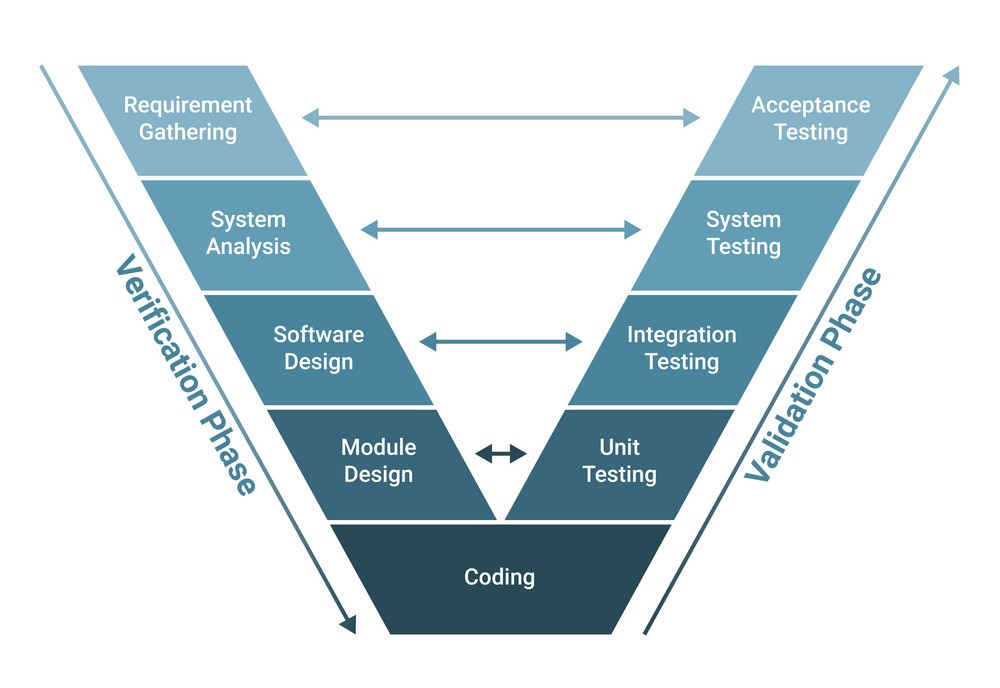
\includegraphics[width=0.7\linewidth]{assets/v-model.jpg}}
    \caption{The V-model software development life cycle \cite{vmodel}}
\end{figure}

The \gls{vmodel} also provides some inspiration for the development methodology of the telemetry system, as frequent
testing and prototyping is a hard requirement. The failure of \glsxtrshort{cuinspace}'s telemetry system in previous
years was due to a lack of continuous testing. This oversight led to a discovery of problems in range testing, which
was never solved and meant that no live telemetry data could be sent during flight. Utilizing the \gls{vmodel} will
require the telemetry system to have frequent prototypes used in testing, which will catch errors earlier in the
development cycle.

In addition to frequent testing, the \gls{vmodel} also prescribes requirements and architecture design to be completed
before implementation. Although this contradicts the \gls{agile} methodology and the nature of development on a student
design team, \glsxtrshort{cuinspace} plans to use this attribute of the \gls{vmodel} to encourage more detailed design
plans as early as possible in the year, before implementation is allowed to progress too far. Having a clearer plan
before the implementation phase begins gives members clearer direction with their tasks and reduces the probability of
having design incompatibilities after implementation is complete, requiring large, last-minute changes.

\subsection{Maintainability}

The \glsxtrshort{cuinspace} telemetry system software must be easily maintainable throughout high turnover of members
and an influx of interested members with limited software development knowledge. This is achieved with detailed
documentation, enforced software standards and division of responsibility between and within the software modules
discussed in \hyperref[s:modules]{section \ref{s:modules}}.

\subsubsection{Documentation}

In order to maintain and enforce detailed documentation of the telemetry system, auto-documentation generation using
Doxygen is enforced. See \hyperref[a:doxygen]{appendix \ref{a:doxygen}} for more information about Doxygen.

All of the software modules use a Doxygen configuration file which outputs warnings when code structures are left
undocumented (functions, C structs, enums, etc.). Doxygen documentation generation is automatically triggered when a
\glsxtrshort{pr} is merged into the module's respective codebase. This ensures that the documentation is always up to
date with the codebase.

In addition to automatic documentation generation on merges, GitHub repositories for the telemetry system modules are
set up to host the static \glsxtrshort{html} website created by Doxygen using \gls{githubpages}. This allows developers
to easily peruse existing documentation without requiring them to download it themselves or render the web-pages
locally.

Doxygen documentation is enforced using the \hyperref[a:javadoc]{JavaDoc style (more information in appendix
    \ref{a:javadoc})}. This style was selected because of its simple syntax, wide selection of information tags and because
it is taught in second year undergraduate engineering courses covering Java programming.

Documentation is required to be written wherever implementation occurs (C files for functions, header files for type
definitions, etc.). This avoids rebuilding all dependent source files when the documentation for a function prototype
is changed in a header file. \cite{doxygen-headers}

In addition to inline documentation for code, all modules mentioned in \hyperref[s:modules]{section \ref{s:modules}}
will come bundled with a help text document which can be invoked in the console with the \texttt{use} command. The help
document will include:

\begin{itemize}
    \setlength{\itemsep}{1pt}
    \setlength{\parskip}{0pt} \setlength{\parsep}{0pt}
    \item The module's version using \gls{semver} notation
    \item A description of the module's purpose
    \item Usage instructions for invocation
    \item A list of all command line options, positional arguments, their default values and the values they accept
    \item Example calls of the module
\end{itemize}

\subsubsection{Code Style}

All code is formatted according to a uniform \hyperref[a:clang-format]{clang-format (see appendix \ref{a:clang-format})
    for more information} configuration. This ensures that code formatting remains readable, and it also ensures that merge
conflicts due to developer formatting differences are avoided. Formatting is enforced via an automatic action on GitHub
which checks that the code adheres to the formatting guidelines before a \glsxtrshort{pr} can be merged.

A comprehensive set of compiler warnings is included in the build system for the telemetry software, which ensures that
common mistakes are caught at compile time (incorrect number of arguments to \texttt{printf}, unused declarations,
etc.). This ensures that code style is kept clean and free of bad practices. Warnings will be visible to developers
whenever they compile.

All code will be linted by GitHub actions using the \gls{qnx} compiler, \texttt{qcc}. This will ensure that compiler
warnings are detected before \glsxtrshort{pr}s are merged, giving developers the ability to fix their code before it
becomes part of the final product.

\subsection{Testing}

The development methodology chosen for the telemetry system places an emphasis on frequent prototyping. Testing is an
important part of the development methodology for validating prototypes continuously.

Developers will be responsible for writing unit tests for features that they implement. Unit tests will be executed
when \glsxtrshortpl{pr} are merged in order to verify that new changes do not break existing functionality. Tests that
are intentionally broken by new changes must come with a justification for the change and a rewrite/removal of the
affected tests.

Integration testing will be performed using shell scripts which can run on the Raspberry Pis. Using shell scripts
allows us to test our program in the real environment it will perform in, on actual hardware, including our
\glsxtrshort{srad} \glsxtrshortpl{pcb} which cannot be emulated in software without a considerable amount of effort.
Additionally, testing modules which are not hardware dependent is not possible automatically using GitHub's actions, as
the \gls{qnx} \glsxtrshort{rtos} kernel is fundamentally incompatible with Docker. \cite{docker-kernel-incompat}


% GLOSSARY %
\pagebreak
\printglossary[title=Glossary]
\printglossary[type=\acronymtype,title=Acronyms]

% BIBLIOGRAPHY %
\pagebreak
\printbibliography

% APPENDIX %
\pagebreak
\appendix

\section{Carleton University InSpace Repositories}

\subsection{Hardware Design}

All of the hardware designs that will be integrated with the telemetry software are available publicly in the
\href{https://github.com/CarletonURocketry/avionics-hardware}{CarletonURocketry avionics-hardware} repository.

\subsection{Telemetry Systems}

\subsubsection{Telemetry Format Specifications} \label{a:telem-format}

All telemetry formatting and encoding specifications, including radio packet format and SD card logging formats, are
visible in the \href{https://github.com/CarletonURocketry/telemetry-format}{CarletonURocketry telemetry-format
    repository}.

\subsubsection{Current Telemetry System} \label{a:cur-system}

All the modules described in this document, their source files, the testing framework and the source files for this
document itself is available in the \href{https://github.com/CarletonURocketry/qnx-stack}{CarletonURocketry qnx-stack
    repository}.

\subsubsection{Previous Telemetry System} \label{a:prev-system}

The repository for the previously used telemetry system is available in the
\href{https://github.com/CarletonURocketry/avionics-software}{CarletonURocketry avionics-software repository}, which is
now available as a public archive.

\subsubsection{Ground Station System} \label{a:ground-station}

The repositories for the ground station system are available below. The ground station repository contains the backend
system for interfacing with the \glsxtrshort{srad} ground station board over serial and decoding radio packets into
human-readable data. The ground station UI repository contains the frontend dashboard used to visualize the telemetry
data in real-time. The two connect over a websocket connection.

\begin{itemize}
    \setlength{\itemsep}{1pt}
    \setlength{\parskip}{0pt} \setlength{\parsep}{0pt}
    \item \href{https://github.com/CarletonURocketry/ground-station}{Ground Station}
    \item \href{https://github.com/CarletonURocketry/ground-station-ui}{Ground Station UI}
\end{itemize}

\section{Referenced Tools and Technologies}

\subsection{Hardware}

\begin{itemize}
    \setlength{\itemsep}{1pt}
    \setlength{\parskip}{0pt} \setlength{\parsep}{0pt}
    \item \href{https://www.raspberrypi.com/products/raspberry-pi-4-model-b/}{Raspberry Pi 4 Model B} \label{a:rpi4}
    \item \href{https://www.segger.com/downloads/jlink/}{SEGGER J-Link} \label{a:jlink}
\end{itemize}

\subsection{Software}

\begin{itemize}
    \setlength{\itemsep}{1pt}
    \setlength{\parskip}{0pt} \setlength{\parsep}{0pt}
    \item \href{https://www.doxygen.nl/index.html}{Doxygen} \label{a:doxygen}
    \item \href{https://www.doxygen.nl/manual/docblocks.html#cppblock}{JavaDoc} \label{a:javadoc}
    \item \href{https://www.segger.com/downloads/jlink/}{OpenOCD}. \label{a:openocd}
    \item \href{https://clang.llvm.org/docs/ClangFormat.html}{clang-format} \label{a:clang-format}
\end{itemize}


\end{document}
